\hypertarget{cogment-core-concepts-guide}{%
\section{Cogment Core Concepts
Guide}\label{cogment-core-concepts-guide}}

Welcome to the Cogment core concepts guide. It contains information that
is pertinent to both the
\href{../cogment/cogment-api-guide.md}{high-level SDK} and the
\href{../cogment/cogment-low-level-api-guide/overview.md}{low-level
API}.

\hypertarget{core-concepts}{%
\subsection{Core Concepts}\label{core-concepts}}

Cogment is built around concepts adapted from multi-agent systems
(agents, environment), Markov decision processes (action and observation
space) and reinforcement learning (trials, rewards).

\hypertarget{trials}{%
\subsubsection{Trials}\label{trials}}

\href{./glossary.md\#trial}{Trials} are what a Cogment deployment runs.
They enable \href{./glossary.md\#actors}{Actors} to interact with their
\href{./glossary.md\#environment}{Environment}. Trials are started by
clients connecting to Cogment. A trial can end either by being
terminated from a client or end by itself, for example once a specific
state of the Environment is reached.

During the trial:

\begin{itemize}
\tightlist
\item
  The \href{./glossary.md\#environment}{Environment} generates
  \href{./glossary.md\#observation}{\textbf{observations}} of its
  internal state and sends them to the
  \href{./glossary.md\#actor}{actors}.
\item
  Given these \href{./glossary.md\#observation}{observations}, each
  \href{./glossary.md\#actor}{actor} might choose and take an
  \href{./glossary.md\#action}{\textbf{action}}.
\item
  The \href{./glossary.md\#environment}{Environment} receives the
  \href{./glossary.md\#action}{actions} and updates its state.
\item
  \href{./glossary.md\#reward}{\textbf{Rewards}} can be sent to the
  \href{./glossary.md\#actor}{actors} from either the environment or
  other actors.
\item
  \href{./glossary.md\#actor}{Actors} receive
  \href{./glossary.md\#reward}{\textbf{rewards}}.
\item
  The \href{./glossary.md\#actor}{actors} or the
  \href{./glossary.md\#environment}{environment} can send
  \href{./glossary.md\#message}{\textbf{messages}} to actors or the
  environment.
\item
  A log of the activity during the trial (observations, actions, rewards
  \& messages) is produced and can be stored.
\end{itemize}

A trial is defined by the participating
\href{./glossary.md\#actor}{Actors} and the host
\href{./glossary.md\#environment}{Environment}. As a concept, Trials are
quite close to Reinforcement Learning (RL)'s \textbf{Episodes}, i.e.~all
the states that come between an initial state and a terminal state.
However, because Cogment can be used outside of an RL context, we prefer
using the more generic term of Trial.

\hypertarget{actors}{%
\subsubsection{Actors}\label{actors}}

\href{./glossary.md\#actor}{Actors} within a trial instantiate
\href{./glossary.md\#actor-class}{actor classes} defined by the nature
of the information they receive from the
\href{./glossary.md\#environment}{environment}, their
\href{./glossary.md\#observation-space}{observation space}, and what
actions they can perform, their
\href{./glossary.md\#action-space}{action space}.

In Cogment, the observation and action space are defined as typed data
structures. In particular, Cogment uses
\href{./glossary.md\#protocol-buffer}{protobuf} as a format to specify
these data structures. This typing defines both an interface contract
between the \href{./glossary.md\#actor}{Actors} and the
\href{./glossary.md\#environment}{Environment} and helps convey semantic
information, thus facilitating the independent design and development of
both.

An \href{./glossary.md\#actor}{Actor} might be controlled either by a
software \href{./glossary.md\#agent}{Agent}, or by a Human. Whichever
the case, the process of generating
\href{./glossary.md\#action}{actions} based on
\href{./glossary.md\#observation}{observations} remains the same, and
the \href{./glossary.md\#environment}{Environment} treats them the same.

\hypertarget{environment}{%
\subsubsection{Environment}\label{environment}}

The \href{./glossary.md\#environment}{Environment} is the context within
which the \href{./glossary.md\#trial}{Trial} takes place. The
Environment receives the \href{./glossary.md\#actions}{actions} done by
the actors, usually updates an internal state, and generates an
\href{./glossary.md\#observation}{observation} for each
\href{./glossary.md\#actor}{Actor}.

The Environment is the main integration point between Cogment and an
external system, either a \textbf{simulation} or a \textbf{real world
system}.

\hypertarget{the-cogment.yaml}{%
\subsection{The cogment.yaml}\label{the-cogment.yaml}}

At the heart of every Cogment project is a \href{https://yaml.org}{YAML}
file typically called \texttt{cogment.yaml}. Its primary role is to
define the \href{./glossary.md\#actor-class}{actor classes} present
within the project, including their
\href{./glossary.md\#action-space}{action} \&
\href{./glossary.md\#observation-space}{observation spaces}, as well as
a default configuration for trials, including the number of actor
participating in each \href{./glossary.md\#trial}{trial} and their class
and implementation.

\hypertarget{architecture}{%
\subsection{Architecture}\label{architecture}}

Running trials with Cogment usually involves the deployment of a cluster
of services and its clients. These components are either provided by the
Cogment framework, depicted below in blue, or implemented for a
particular project, depicted below in orange.

\begin{figure}
\centering
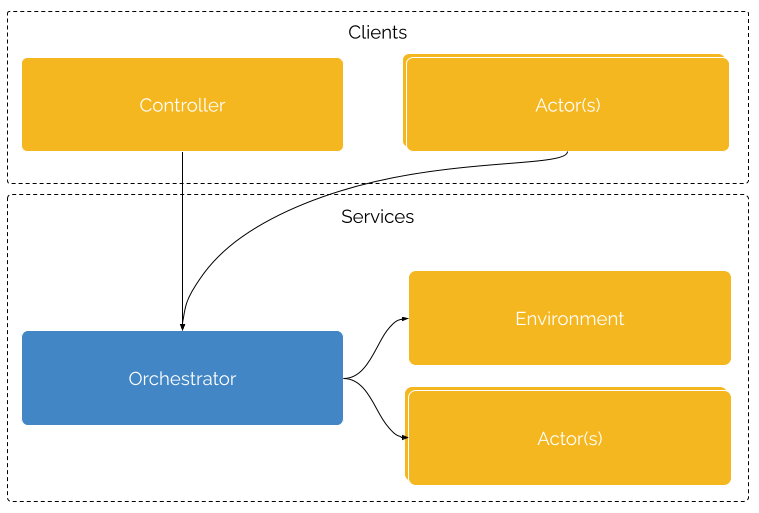
\includegraphics{./cogment_architecture_simple.png}
\caption{Cogment Architecture - Simple}
\end{figure}

User implemented components use one of the
\href{../cogment/cogment-api-guide.md}{Cogment SDKs} or directly
implement the
\href{../cogment/cogment-low-level-api-guide/overview.md}{underlying
protocol}. Components communicate using \href{https://grpc.io}{gRPC},
clients can also communicate in a web-friendly way using
\href{https://grpc.io/docs/platforms/web/}{gRPC-Web} and
\href{https://github.com/improbable-eng/grpc-web/tree/master/go/grpcwebproxy}{grpcwebproxy}.

\hypertarget{orchestrator}{%
\subsubsection{Orchestrator}\label{orchestrator}}

The Orchestrator is the glue that binds everything together. It is
responsible for running the \href{./glossary.md\#trial}{trials} and
contacting other services as needed to ensure their execution.

The key aspect of Cogment's orchestrator is its capacity to handle a
number of network connections in parallel while keeping its
responsiveness.

\hypertarget{controller}{%
\subsubsection{Controller}\label{controller}}

The Controller is a key part of using Cogment, it initiates
communication with the Orchestrator to control the execution of
\href{./glossary.md\#trial}{trials}. It is responsible for starting
\href{./glossary.md\#trial}{Trials}, retrieving and watching their state
(including the end of the trial), or requesting trial termination.

\hypertarget{environment-1}{%
\subsubsection{Environment}\label{environment-1}}

The Environment implementation is accessed by the
\href{./glossary.md\#orchestrator}{Orchestrator} to run the
\href{./glossary.md\#environment}{Environment} during
\href{./glossary.md\#trial}{Trials}.

Using one of \href{../cogment/cogment-api-guide.md}{Cogment's SDKs}, the
Environment can be implemented as a function integrating a \emph{``state
of the world''} with the \href{./glossary.md\#trial}{Trial}. This
function performs the following tasks during the Trial:

\begin{itemize}
\tightlist
\item
  Generate \href{./glossary.md\#observation}{Observations} from the
  current \emph{state of the world}, for example retrieving the visible
  objects from a 3D simulation.
\item
  Apply the \href{./glossary.md\#action}{Actions}, thus updating the
  \emph{state of the world}, for example changing the velocity of a
  moving vehicle in a race simulation.
\item
  Evaluate the performance of \href{./glossary.md\#actor}{Actors} and
  send them \href{./glossary.md\#reward}{Rewards}, for example by
  checking if a vehicle crossed the finish line in a race simulation.
\item
  Send and receive direct messages.
\end{itemize}

\hypertarget{actors-1}{%
\subsubsection{Actors}\label{actors-1}}

Actors can be implemented in two different ways, either as a service or
as a client. \textbf{Service Actor} implementations are accessed by the
\href{./glossary.md\#orchestrator}{Orchestrator} during
\href{./glossary.md\#trial}{Trials}, while \textbf{Client Actor}
implementations join a Trial by initiating the communication with the
Orchestrator. Client Actors implementations can \emph{reach} a Cogment
deployment through
\href{https://en.wikipedia.org/wiki/NAT_traversal}{NAT traversal}. This
makes them particularly well-suited to implement human-driven Actors, in
web-browsers for example.

Using one of \href{../cogment/cogment-api-guide.md}{Cogment's SDKs}
Actors can be implemented as functions handling the integration between
a decision-making Actor (\href{./glossary.md\#agent}{software agent} or
Human) and the \href{./glossary.md\#trial}{Trial}. This function
performs the following tasks during the Trial:

\begin{itemize}
\tightlist
\item
  Receive \href{./glossary.md\#observation}{Observations} and do
  \href{./glossary.md\#action}{Actions} in response, for example
  vectorizing the retrieved observation, feeding it to a neural network
  and converting its output to an Action.
\item
  Receive \href{./glossary.md\#reward}{Rewards}, for example using them
  to update a neural network.
\item
  Send and receive direct messages.
\end{itemize}

Please note that rewards can also be retrieved after the fact using an
\protect\hyperlink{additional-optional-services}{activity logger}.

\hypertarget{additional-optional-services}{%
\paragraph{Additional optional
services}\label{additional-optional-services}}

Beyond the core services described above, a Cogment deployment can
include these additional ones:

\begin{itemize}
\tightlist
\item
  \textbf{Pre trial hooks} can be used to dynamically setup Trials from
  a given configuration, for example changing the number of Actors or
  pointing to other Environment or Actor implementations.
\item
  \textbf{Activity Logger} can be used to listen to the activity during
  a trial (actions, observations, rewards, messages), for example, to do
  store these data in order to do offline training of AI agents.
\end{itemize}
